% !TEX root = ../sethomas_thesis_main.tex
\documentclass[border=1mm,
               class=article
               preview]{standalone}
\usepackage{tikz}
\begin{document}
\begin{tikzpicture}
    \pgfmathsetmacro{\YDelta}{1.1};%Offset for adding the side view

    \pgfmathsetmacro{\xLegendTop}{0.2};
    \pgfmathsetmacro{\yLegendTop}{5.3+\YDelta};

    \pgfmathsetmacro{\xLegendBottom}{1.1}; \pgfmathsetmacro{\yLegendBottom}{2.6+\YDelta};

    \pgfmathsetmacro{\xLegendSide}{0.2}; \pgfmathsetmacro{\yLegendSide}{0.65}

    % \node[anchor=south west,inner sep=0] (graph) at (0,0){\includegraphics[width=0.4\textwidth]{img/mechanism_iso_axes.png}};
    \node[anchor=south west,inner sep=0] (graph) at (0,0){\includegraphics[width=0.4\textwidth]{images/chap7/mechanism_iso_axes_side.png}};
    \begin{scope}[x={(graph.south east)},y={(graph.north west)}]
        \node[align=left] at (0.04,0.742) {\footnotesize x};
        \node[align=left] at (0.15,0.735) {\footnotesize y};
        \node[align=left] at (0.06,0.85) {\footnotesize z};

        \node[align=left] at (0.095,0.445) {\footnotesize x};
        \node[align=left] at (0.155,0.345) {\footnotesize y};
        \node[align=left] at (0.045,0.34) {\footnotesize z};

        \node[align=left] at (0.03,0.1) {\footnotesize x};
        \node[align=left] at (0.135,0.1) {\footnotesize y};
        \node[align=left] at (0.08,0.155) {\footnotesize z};
    \end{scope}

    \pgfmathsetmacro{\xStartLine}{\xLegendSide-0.2};
    \pgfmathsetmacro{\xStopLine}{\xLegendSide+7};
    \draw[densely dotted] (\xStartLine,\yLegendSide-0.17) -- (\xStopLine,\yLegendSide-0.17);
    \node[align=left] at (\xStopLine+0.3,\yLegendSide-0.14) {\small $L_1$};
    \draw[densely dotted] (\xStartLine,\yLegendSide-0.37) -- (\xStopLine,\yLegendSide-0.37);
    \node[align=right] at (\xStartLine-0.3,\yLegendSide-0.34) {\small $L_2$}; %,draw,circle,inner sep=0.1pt
    \draw[densely dotted] (\xStartLine,\yLegendSide-0.57) -- (\xStopLine,\yLegendSide-0.57);
    \node[align=left] at (\xStopLine+0.3,\yLegendSide-0.6) {\small $L_3$};

    \pgfmathsetmacro{\xZOOM}{7.4};
    \pgfmathsetmacro{\yZOOM}{7.2};
    \node[anchor=north east,inner sep=0] (graph) at (\xZOOM,\yZOOM){\includegraphics[width=2.5cm]{images/chap7/pivot.pdf}};
    \node[align=left] at (\xZOOM-1.,\yZOOM-0.45) {$e$};
    \node[align=left] at (\xZOOM-0.4,\yZOOM-1.3) {$b$};
    \node[align=left] at (\xZOOM-1.7,\yZOOM-1) {$r$};
    % \draw[help lines] (0,0) grid (8,8); % $$$$$$$$$$$$$ HELPS A LOT FOR COORDINATES $$$$$$$
\end{tikzpicture}
\end{document}
